
\chapter {\noun{Use cases}}
We define two groups of actors - clients like patients, doctors and pharmacists which benefit from the system on daily basis and third parties - administrators, analytic tools and goverment authorities which cope with the system on special ocassions.

\begin{figure}[h]
\centering
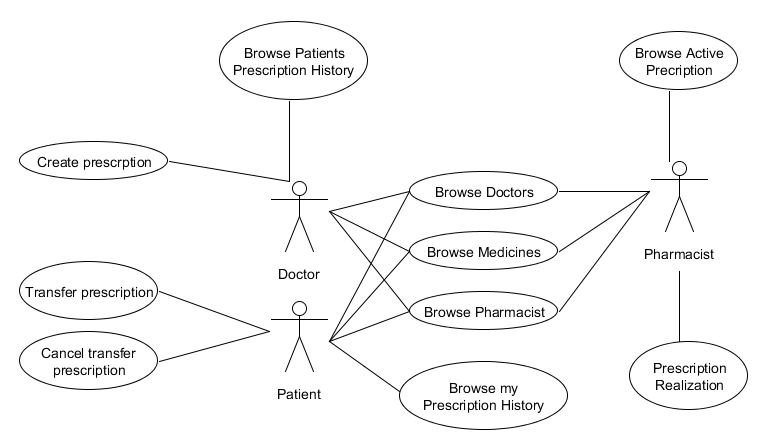
\includegraphics[width=1\textwidth]{database/standardUseCases.png}
\end{figure} 

Every use case requires the users to establish secure channel of communication with central server and have to be logged in which will be described more thorougly in section~\ref{sec:login}.
\section{Shared use cases}

Three use cases are applicable for patient, pharmacist and doctors and they consider browsing informations which can be publicly accessible, that is:
\begin{packed_enum}
\item Browse Doctors
\item Browse Medicines 
\item Browse Pharmacists
\end{packed_enum}
Rest of use cases which are applicable to only one actor is described in their respective subsections.
\small
\begin{longtable}{|p{6cm}|p{7.75cm}|}
   
    \hline
    Actors: Patient, Doctor, Pharmacist &Title: Browse Doctors \\ \hline
    Goal: & Allows to find doctor with specific name, address or license number. \\ \hline
    Scenario: & User enters any or all of name, address and license number of searched doctor. \\ \hline
    Result: & List of doctors corresponding to the query. \\ \hline
    Database  method: & \texttt{browse\_doctors} \\ \hline
    
\end{longtable}

\begin{longtable}{|p{6cm}|p{7.75cm}|}
    
    \hline
    Actors: Patient, Doctor, Pharmacist &Title: Browse Pharmacies \\ \hline
    Goal: & Allows to find pharmacist and pharmacy with specific name, address or license number. \\ \hline
    Scenario: & User enters any or all of name, address, license number of searched pharmacist or pharmacy name. \\ \hline
    Result: & List of pharmacists corresponding to the query. \\ \hline
    Database  method: & \texttt{browse\_pharmacies} \\ \hline

\end{longtable}


    \begin{longtable}{| p{6cm} | p{7.75cm} |}
    \hline
    Actors: Patient, Doctor, Pharmacist &Title: Browse Medicines \\ \hline
    Goal: & Allows to find medicine with specific name or type. \\ \hline
    Scenario: & User enters name or/and type of medicine he is searching. \\ \hline
    Result: & List of medicines corresponding to the query. \\ \hline
    Database  method: & \texttt{browse\_medicines} \\ \hline
    \end{longtable}

\normalsize

\section{\noun{Patient}}

\small
    \begin{longtable}{| p{6cm} | p{7.75cm} |}
    \hline
    Actors: Patient &Title: Transfer prescription \\ \hline
    Goal: & Allows to transfer a prescription to another patient and give him credentials to realize this prescription. Patient who transferred the prescription losses his right to realize it by himself. If he wants the prescription back he has to cancel the transfer (next use case). \\ \hline
    Scenario: & Patient enters his id, id of new owner, the prescription id he wants to transfer and his signature. \\ \hline
    Result: & OK response from database and iId of new owner of prescription. \\ \hline
    Database  method: & \texttt{transfer\_prescription} \\ \hline
\end{longtable}

    \begin{longtable}{| p{6cm} | p{7.75cm} |}
    \hline
    Actors: Patient &Title: Cancel Transfer Prescription \\ \hline
    Goal: & Allows to revert transfering of prescription to another patient. \\ \hline
    Scenario: & Patient enters his id, prescription id he wants transfers to revert and his signature. \\ \hline
    Result: & OK response from database. \\ \hline
    Database  method: & \texttt{cancel\_prescription\_transfer} \\ \hline
\end{longtable}

    \begin{longtable}{| p{6cm} | p{7.75cm} |}
    \hline
    Actors: Patient &Title: Browse My Prescriptions History \\ \hline
    Goal: & Patient can see his history of realized and created prescriptions.\\ \hline
    Scenario: & Patient sends his id which is signed by his key from smartcard. Patient can define the time span of returned prescriptions as also a filter to only return prescriptions which aren't realized yet. \\ \hline
    Result: & List of prescriptions for the patient. \\ \hline
    Database  method: & \texttt{browse\_prescription\_history} \\ \hline

\end{longtable}

\normalsize
\newpage
\section{\noun{Doctor}}

\small
    \begin{longtable}{| p{6cm} | p{7.75cm} |}
    \hline
   Actors:  Doctor &Title: Create prescription \\ \hline
    Goal: & Allows to create a new prescription in database for selected patient..\\ \hline
    Scenario: & Doctor enters his and patients ids, as well as the data specific to the medicine - id, dosage, unit and quanitity. Everything is signed by his key. \\ \hline
    Result: & OK response from database. \\ \hline
    Database  method: & \texttt{create\_prescription} \\ \hline
    \end{longtable}



    \begin{longtable}{| p{6cm} | p{7.75cm} |}
    \hline
    Actors: Doctor &Title: Browse Patients Prescriptions History \\ \hline
    Goal: & Doctor can see patient history of realized and created prescriptions..\\ \hline
    Scenario: & Doctor sends his id - he will see all prescriptions created by him. If he will add the id of patient with patients signature, he will see the full history of prescriptions of current patient. Doctor can define the time span of returned prescriptions as also a filter to only return prescriptions which aren't realized yet. \\ \hline
    Result: & List of prescriptions for the patient. \\ \hline
    Database  method: & \texttt{browse\_patient\_prescription\_history} \\ \hline
    \end{longtable}
\normalsize

\section{\noun{Pharmacist}}

\small
    \begin{longtable}{| p{6cm} | p{7.75cm} |}
    \hline
    Actors: Pharmacist &Title: Prescription realization\\ \hline
    Goal: & Pharmacist realizes the prescription. DB checks if the request can be verified and if the prescription is valid.\\ \hline
    Scenario: & Pharmacist enters his id, prescription id as well as drugs id, dosage and qunatity of medicine. Everything is signed by pharmacist key. \\ \hline
    Result: & OK response from database if operation was successful. \\ \hline
    Database  method: & \texttt{prescription\_realization} \\ \hline
    \end{longtable}



    \begin{longtable}{| p{6cm} | p{7.75cm} |}
    \hline
    Actors: Pharmacist &Title: Browse Active Prescriptions \\ \hline
    Goal: & Pharmacist can see prescriptions which are not yet realized. \\ \hline
    Scenario: & Pharmacist sends his id and id of current patient which are signed by both of their keys. Pharmacist can see only prescriptions which are not yet realized. \\ \hline
    Result: & List of prescriptions for the patient. \\ \hline
    Database  method: & \texttt{browse\_active\_prescriptions} \\ \hline
    \end{longtable}

\normalsize
\section{\noun{Special Users}}

There are also defined three other users which cope with the system on special ocassions.
These are - administrator, which maintains the system, analytic tools which can be used to obtain statistical data and the goverment authority which has super access to all the data after acquiring proper permissions from court or police.

\begin{figure}[h]
\begin{center}
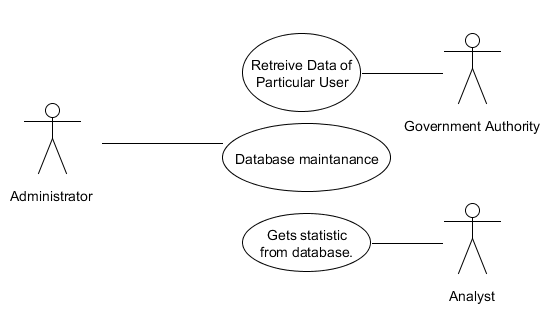
\includegraphics[width=0.7\textwidth]{database/specialUseCases.png}
\end{center}
\end{figure} 

\small
    \begin{longtable}{| p{6cm} | p{7.75cm} |}
    \hline
    Actor: Administrator &Title: Central Server maintenance \\ \hline
    Goal: & Administrator modifies the database, upgrades software etc. \\ \hline
    \end{longtable}


\newpage
    \begin{longtable}{| p{6cm} | p{7.75cm} |}
    \hline
    Actor: Goverment Authority &Title: Retreive Data Of Particular User \\ \hline
    Goal: & Goverment Authority (GA) can retreive all sensitive data of every user after showing permission to do so e.g. court order. GA account password can be separated into several pieces to ensure that one attacker won't be in possesion of the key. \\ \hline
    \end{longtable}



    \begin{longtable}{| p{6cm} | p{7.75cm} |}
    \hline
    Actor: Analytic tools &Title: Obtaining statistics from DB \\ \hline
    Goal: & Analyst can query the database for statistical data e.g. number of medicines sold in last month. Analyst can't query patients or link prescriptions data to particular person. \\ \hline
    \end{longtable}

\normalsize
